\documentclass[10pt,a4paper]{article}
\usepackage[margin=2cm]{geometry}
\usepackage{booktabs,graphicx,float}
\usepackage[T1]{fontenc}
\setlength{\parindent}{0pt}\setlength{\parskip}{0.4em}
\newcommand{\src}[1]{{\footnotesize\emph{Source: \texttt{#1}}}}
\title{Kinect Lite: Results (depth-only ICP)}
\date{}
\begin{document}
\maketitle
Two depth cleaners are compared: our \textbf{9$\times$9 median} and the \textbf{paper} (Fu et al., 2012). Each cleaned sequence is tracked with depth-only ICP and the camera path is compared with the true path. ATE is total drift (cm), RPE the error per step (mm); lower is better. Datasets: ICL-NUIM living room kt0 (150 tracked frames) and TUM RGB-D fr3 long\_office\_household (150 tracked frames).

\section*{1. Depth accuracy (ICL, against the true depth)}
\begin{center}
\begin{tabular}{lcccc}\toprule
Method & MAE (mm) & RMSE (mm) & Median err (mm) & Within 1 cm\\\midrule
No cleaning & 39.2 & 187.5 & 13.3 & 42.2\%\\
Median 9$\times$9 & \textbf{18.8} & \textbf{55.4} & \textbf{12.3} & \textbf{44.7\%}\\
Paper & 37.7 & 186.0 & 13.4 & 33.7\%\\\bottomrule
\end{tabular}\\[2pt]\src{src/results/icl\_compare.txt}
\end{center}
\begin{figure}[H]\centering
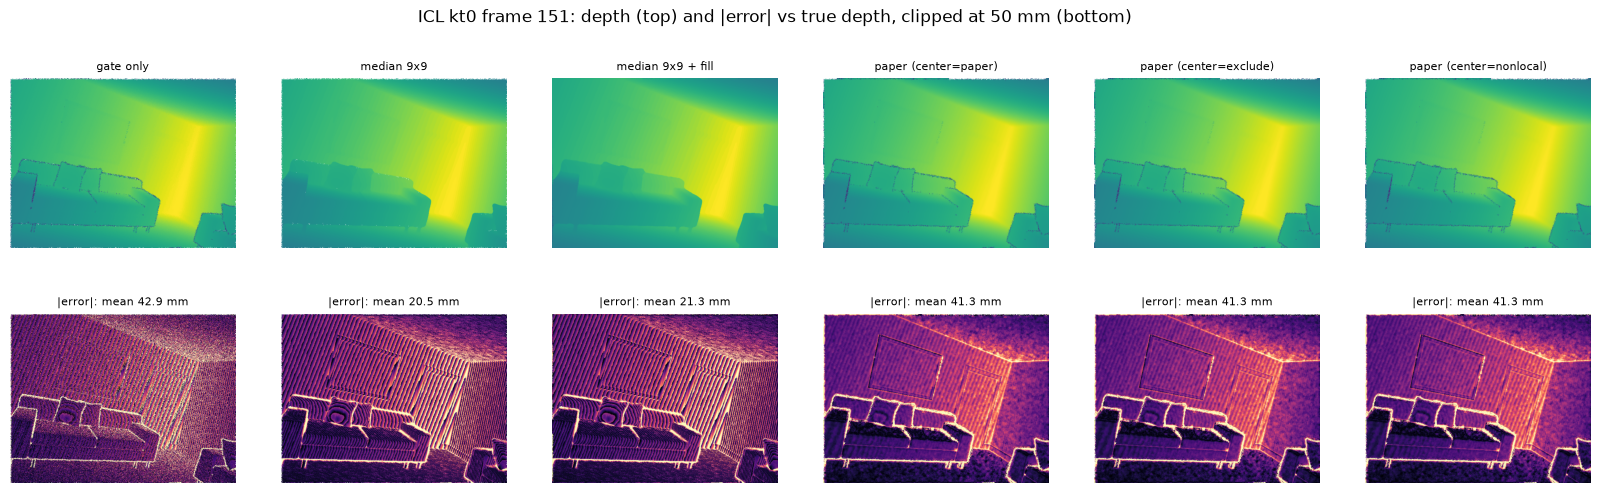
\includegraphics[width=\textwidth]{../src/results/icl_depth_example.png}
\caption{ICL frame 151: cleaned depth (top) and error against the true depth (bottom).}
\end{figure}

\section*{2. Camera tracking with point-to-plane ICP}
\begin{center}
\begin{tabular}{lcc}\toprule
Method (ATE / RPE) & ICL & TUM\\\midrule
True depth & 0.19 / 0.07 & --\\
No cleaning & 17.07 / 14.43 & 13.97 / 11.69\\
Median 9$\times$9 & 14.94 / 11.78 & 13.32 / 10.86\\
Paper & \textbf{0.95 / 2.02} & \textbf{3.33 / 4.37}\\\bottomrule
\end{tabular}\\[2pt]\src{src/results/icl\_compare.txt, tum\_compare.txt}
\end{center}
The paper has the worse per-pixel depth error but tracks about 6$\times$ better per step.
\begin{figure}[H]\centering
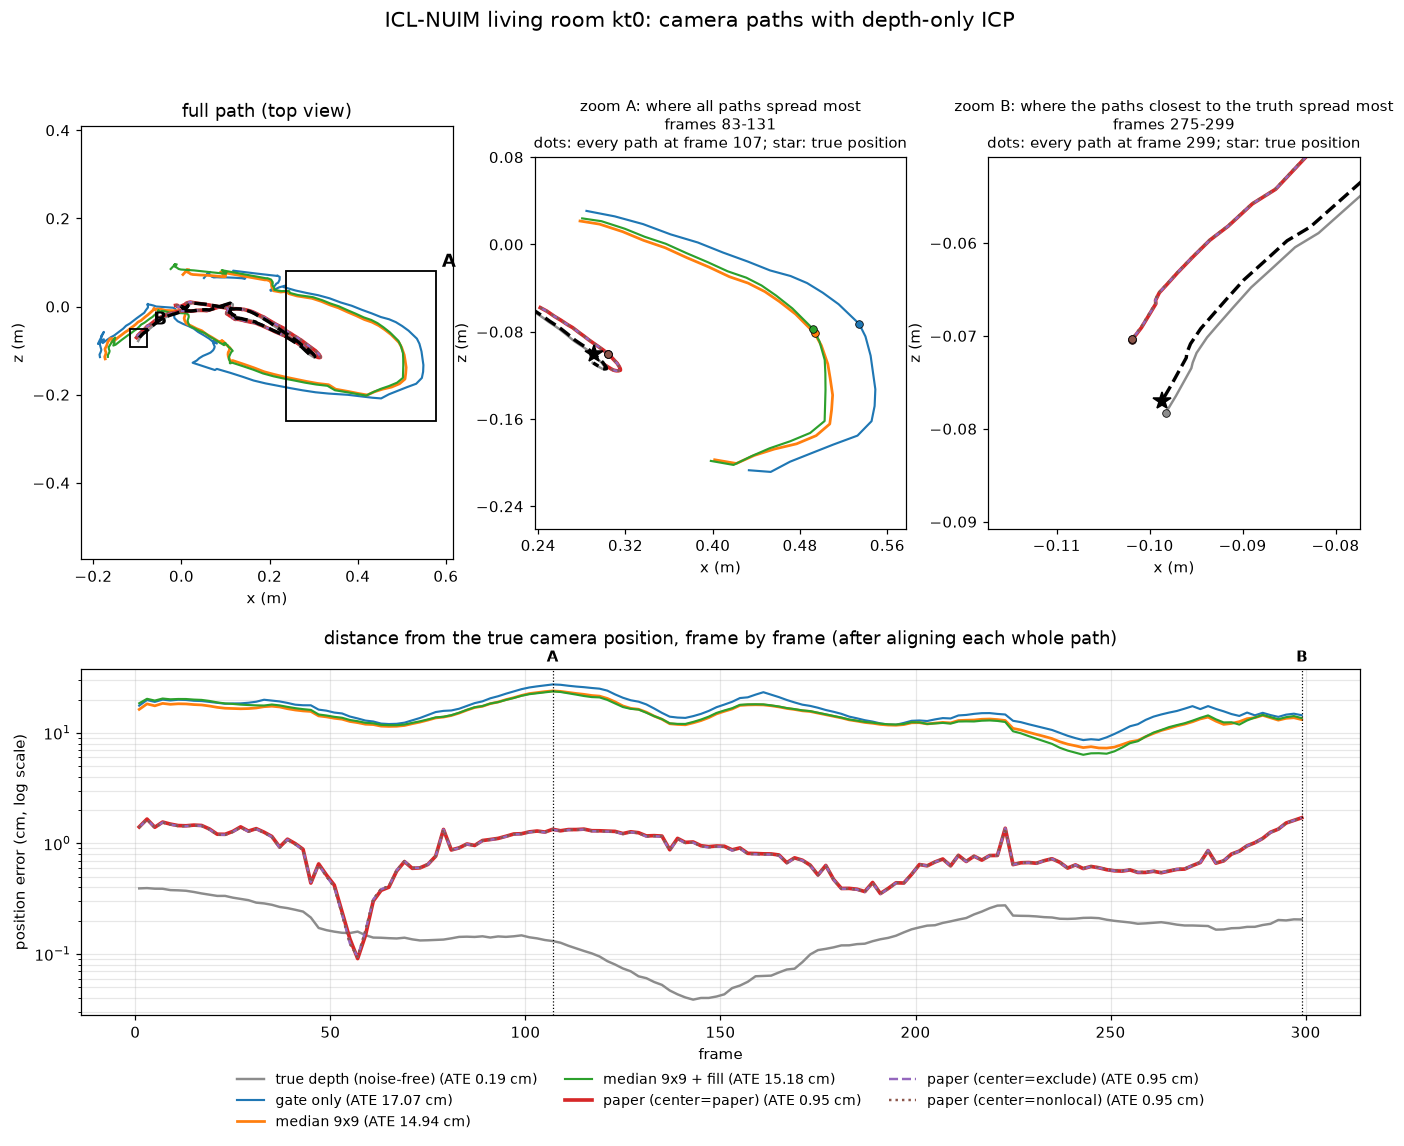
\includegraphics[width=0.9\textwidth]{../src/results/icl_paths_depth_zoom.png}
\caption{ICL: estimated camera paths (top) and position error per frame (bottom).}
\end{figure}
\begin{figure}[H]\centering
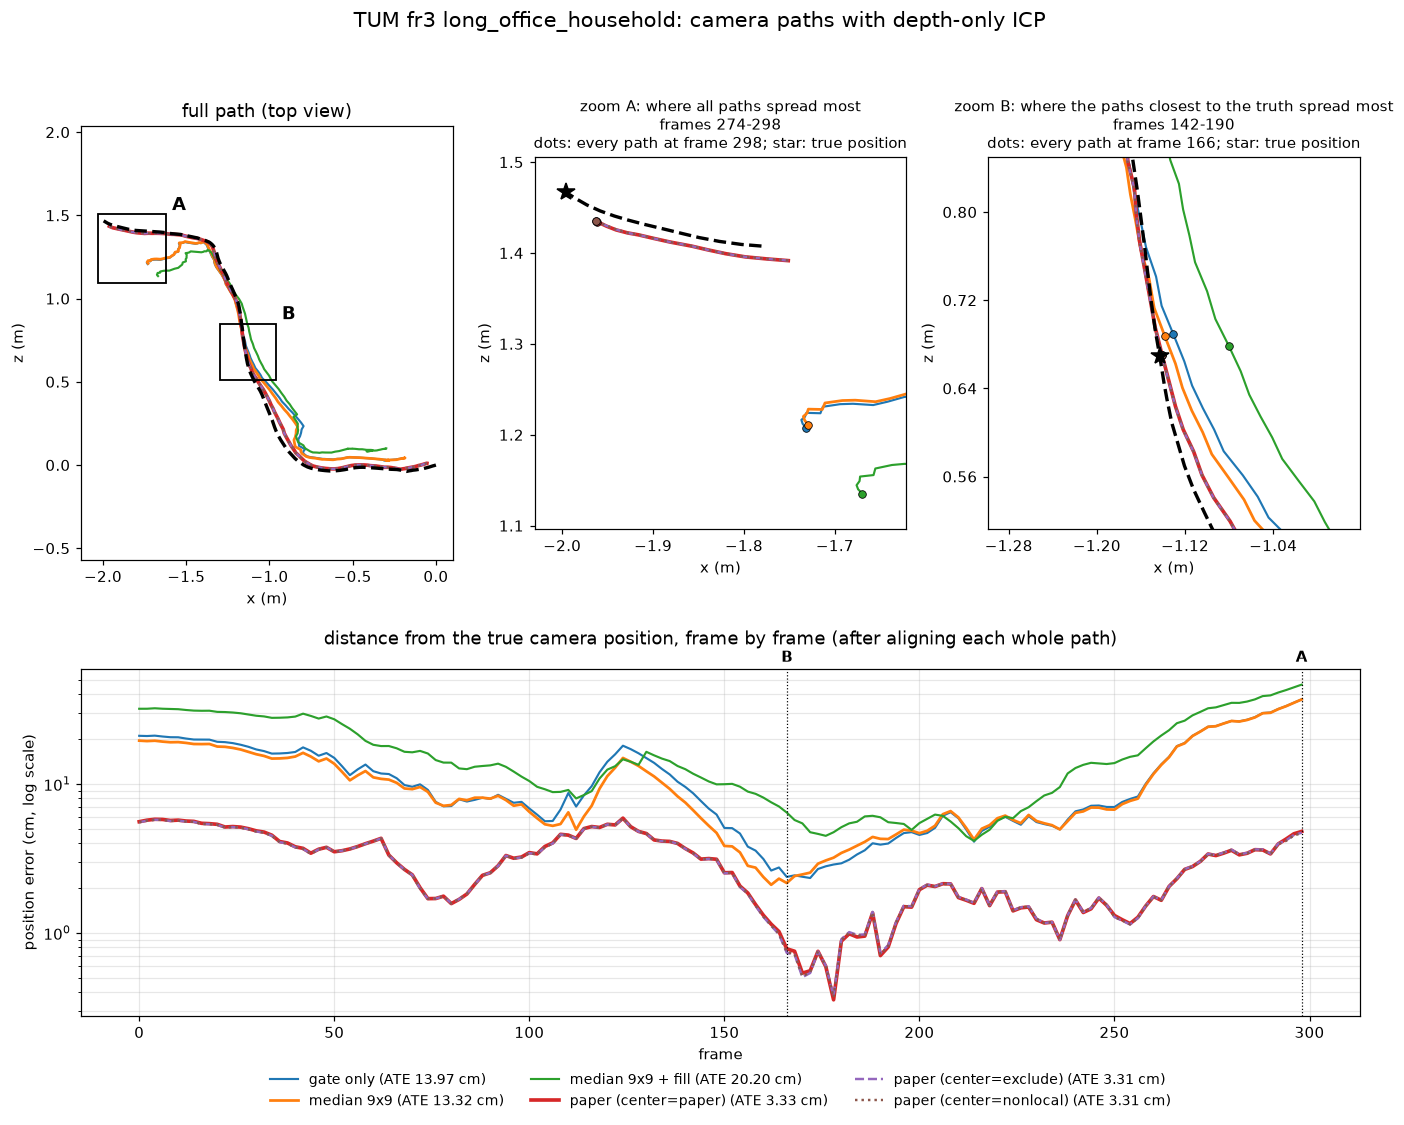
\includegraphics[width=0.9\textwidth]{../src/results/tum_paths_depth_zoom.png}
\caption{TUM: estimated camera paths (top) and position error per frame (bottom).}
\end{figure}

\section*{3. ICP variants (ATE / RPE)}
\begin{center}
\small
\begin{tabular}{llcccc}\toprule
 & Depth & Point-to-point & Point-to-plane & Plane + Tukey & GICP\\\midrule
ICL & True depth & 1.81 / 3.29 & 0.19 / 0.07 & 0.14 / 0.05 & --\\
 & No cleaning & 36.96 / 21.36 & 17.05 / 14.38 & 22.47 / 17.47 & --\\
 & Median & 28.50 / 19.72 & 14.94 / 11.78 & 19.24 / 14.11 & --\\
 & Paper & 1.93 / 3.16 & 0.95 / 2.02 & 1.42 / 2.54 & --\\\midrule
TUM & No cleaning & 27.24 / 14.92 & 13.97 / 11.69 & 14.31 / 11.55 & --\\
 & Median & 18.14 / 13.78 & 13.33 / 10.86 & 13.07 / 10.96 & diverged\\
 & Paper & 5.31 / 5.21 & 3.33 / 4.37 & 3.21 / 4.23 & 14.13 / 43.42\\\bottomrule
\end{tabular}\\[2pt]\src{src/results/icp\_variants.txt}
\end{center}
Point-to-plane beats point-to-point in all seven rows. The robust Tukey loss gives no clear gain. The paper beats the median under every variant that ran. Generalized ICP produced non-finite poses on noisy depth (no ICL numbers; TUM median diverged) and was not tuned. The numbers come from the log of a Kaggle run that crashed at the final table step, after all other tracking had finished.

\section*{4. Why the median does not help ICP (9 ICL frames)}
\begin{center}
\begin{tabular}{lcccc}\toprule
 & \multicolumn{2}{c}{Normal error vs true (deg)} & \multicolumn{2}{c}{Consecutive-frame disagreement (mm)}\\
 & median & mean & median $|r|$ & bias\\\midrule
True depth & -- & -- & 0.3 & 0.01\\
No cleaning & 5.5 & 10.1 & 5.0 & 0.84\\
Median & 2.8 & 7.4 & 3.6 & 1.09\\
Paper & \textbf{1.6} & \textbf{3.7} & \textbf{1.8} & \textbf{0.26}\\\bottomrule
\end{tabular}\\[2pt]\src{experiments/normals\_check/results/normals.txt}
\end{center}
The paper's normals are about twice as accurate and its consecutive frames agree about twice as well. The check uses 9 frames on ICL only and cannot separate smoothing from temporal averaging.

\section*{5. Hole filling (ATE in cm, depth-only ICP)}
\begin{center}
\small
\begin{tabular}{lcccc}\toprule
Fill method & Fill err (mm) & ICL & TUM & Time/frame\\\midrule
None (keep holes) & -- & \textbf{14.94} & 13.33 & 0 ms\\
Telea inpainting & 87.0 & 15.18 & 20.21 & 210 ms\\
Navier--Stokes & 22.5 & 15.36 & \textbf{12.03} & 224 ms\\
Nearest pixel & 22.3 & 15.05 & 17.54 & 50 ms\\
Region growing (small holes) & 15.5 & 14.94 & 13.32 & 52 ms\\
Region growing (median) & 22.5 & 15.15 & 15.14 & 386 ms\\
Background & 83.1 & 15.24 & 13.51 & 40 ms\\
Temporal (paper) & \textbf{12.2} & 15.11 & 13.37 & 7.9 s\\\bottomrule
\end{tabular}\\[2pt]\src{experiments/hole\_filling/results/fills.txt}
\end{center}
No fill reliably improves tracking. The one gain (Navier--Stokes on TUM) does not hold on ICL.
\begin{figure}[H]\centering
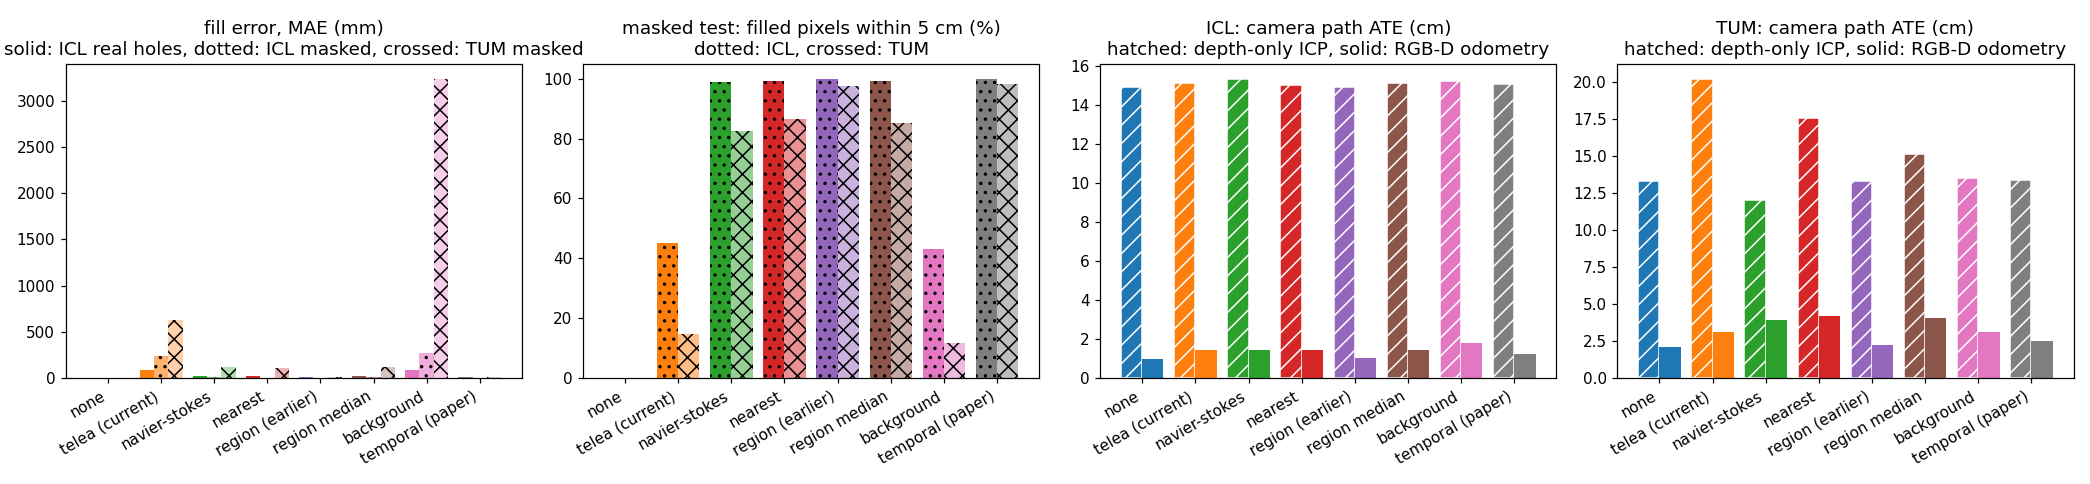
\includegraphics[width=\textwidth]{../experiments/hole_filling/results/fills.png}
\caption{Hole-filling comparison. The tracking panels in this figure were produced by an earlier version of the script that also showed another tracker; the depth-only ICP values are those in the table above.}
\end{figure}
\end{document}
